\nocite{anleitungV703}
\section{Auswertung}
\label{sec:Auswertung}
\subsection{Geiger-Müller Kennlinie}
Zunächst sind die Zählraten zu den entsprechenden Beschleunigungsspannungen $U$ in der Tabelle {\ref{tab:Kennlinie}}
aufgelistet. Anhand dieser Tabelle wird der Arbeitspunkt bei $U_{\text{A}} = 560\,\unit{\volt}$ bestimmt. 
\begin{table}[H]
  \centering
  \caption{Messdaten zur Bestimmung der Geiger-Müller Kennlinie bei einer Messzeit von $60\,\unit{\second}$.}
  \label{tab:Kennlinie}
  \begin{tblr}{colspec={c c  c| c c c}}
      \toprule
      $U\,[\unit{\volt}]$ & $N\,[\unit{(60\,\second)^{-2}}]$ & $N\,[\unit{\second^{-2}}]$ &  $U\,[\unit{\volt}]$ & $N\,[\unit{(60\,\second)^{-2}}]$ & $N\,[\unit{\second^{-2}}]$ \\
      \midrule
      300 & 0     & 0      & 560 & 16739 & 278,98\\
      320 & 0     & 0      & 580 & 16600 & 276,67\\
      340 & 15594 & 259,90 & 600 & 16674 & 277,90\\
      360 & 15904 & 265,07 & 620 & 17050 & 284,17\\
      380 & 16267 & 271,12 & 640 & 16914 & 281,90\\
      400 & 16297 & 271,62 & 660 & 17245 & 287,42\\
      420 & 16369 & 272,82 & 680 & 17223 & 287,05\\
      440 & 16456 & 274,27 & 700 & 17173 & 286,22\\
      460 & 16458 & 274,30 & 720 & 17699 & 294,98\\
      480 & 16426 & 273,77 & 740 & 18787 & 313,12\\
      500 & 16705 & 278,42 & 760 & 19890 & 331,50\\
      520 & 16769 & 279,48 & 780 & 21871 & 364,52\\
      540 & 16632 & 277,20  &    &     & \\
      \bottomrule
  \end{tblr}
\end{table}
Diese Messwerte sind in der Abbildung (\ref{fig:Kennlinie_Plot}) abgebildet. Zusätzlich ist der Arbeitspunkt markiert und eine lineare Regression für die Plateausteigung
ist dargestellt. Graphisch wird eine Plateaulänge von $320\,\unit{\volt}$ abgelesen. Die Ausgleichsgerade wird mithilfe der Funktion $y = mx+b$ bestimmt. Daraus ergeben sich die Werte
\begin{align*}
  m &= (0,049\pm0,005)\,\unit[per-mode=fraction]{\per\volt\per\second}\\
  b &= (251,8\pm2,7)\,\unit[per-mode=fraction]{\per\second}\,.
\end{align*}
Demnach lautet die Plateausteigung 
$$m_{\text{Plateau}} = (1,77\pm0,17)\,\unit[per-mode=fraction]{\percent\per100\,\volt}\,.$$
\begin{figure}[H]
  \centering
  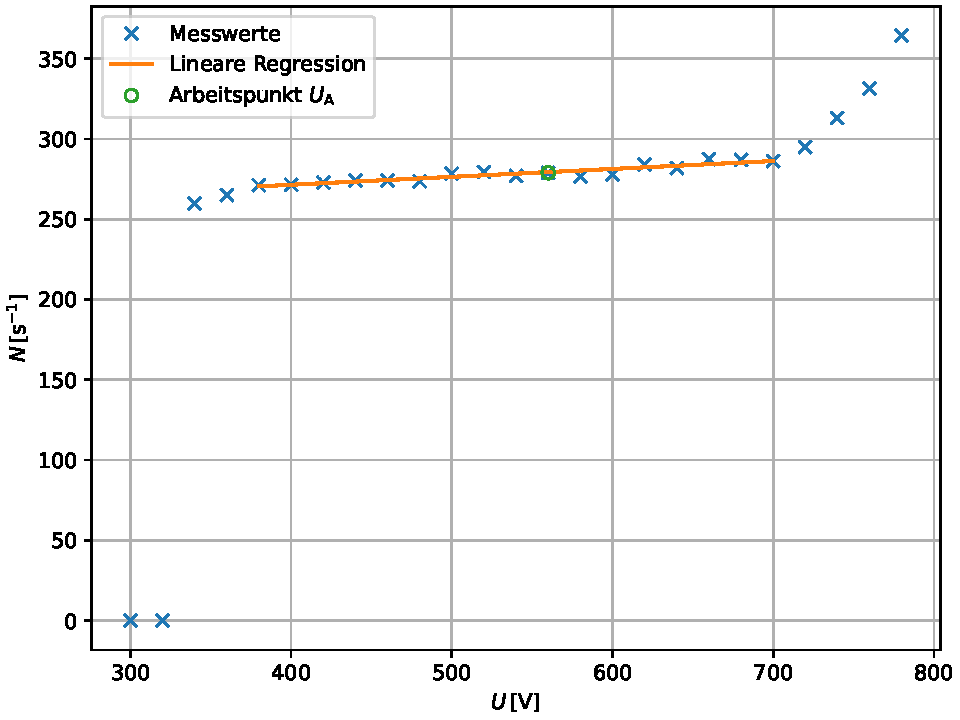
\includegraphics[width=0.8\textwidth]{Kennlinie.pdf}
  \caption{Messdaten mit dem Arbeitspunkt $U_{\text{A}}$ und eine lineare Regression für die Plateausteigung.}
  \label{fig:Kennlinie_Plot}
\end{figure}

\subsection{Bestimmung der Totzeit}
Anhand der Abbildung des Oszilloskops \ref{fig:Totzeit_Oszilloskop} wird die Totzeit $\tau _{\text{Oszilloskop}} = 225\,\unit{\micro\second}$
ermittelt.
\begin{figure}[H]
  \centering
  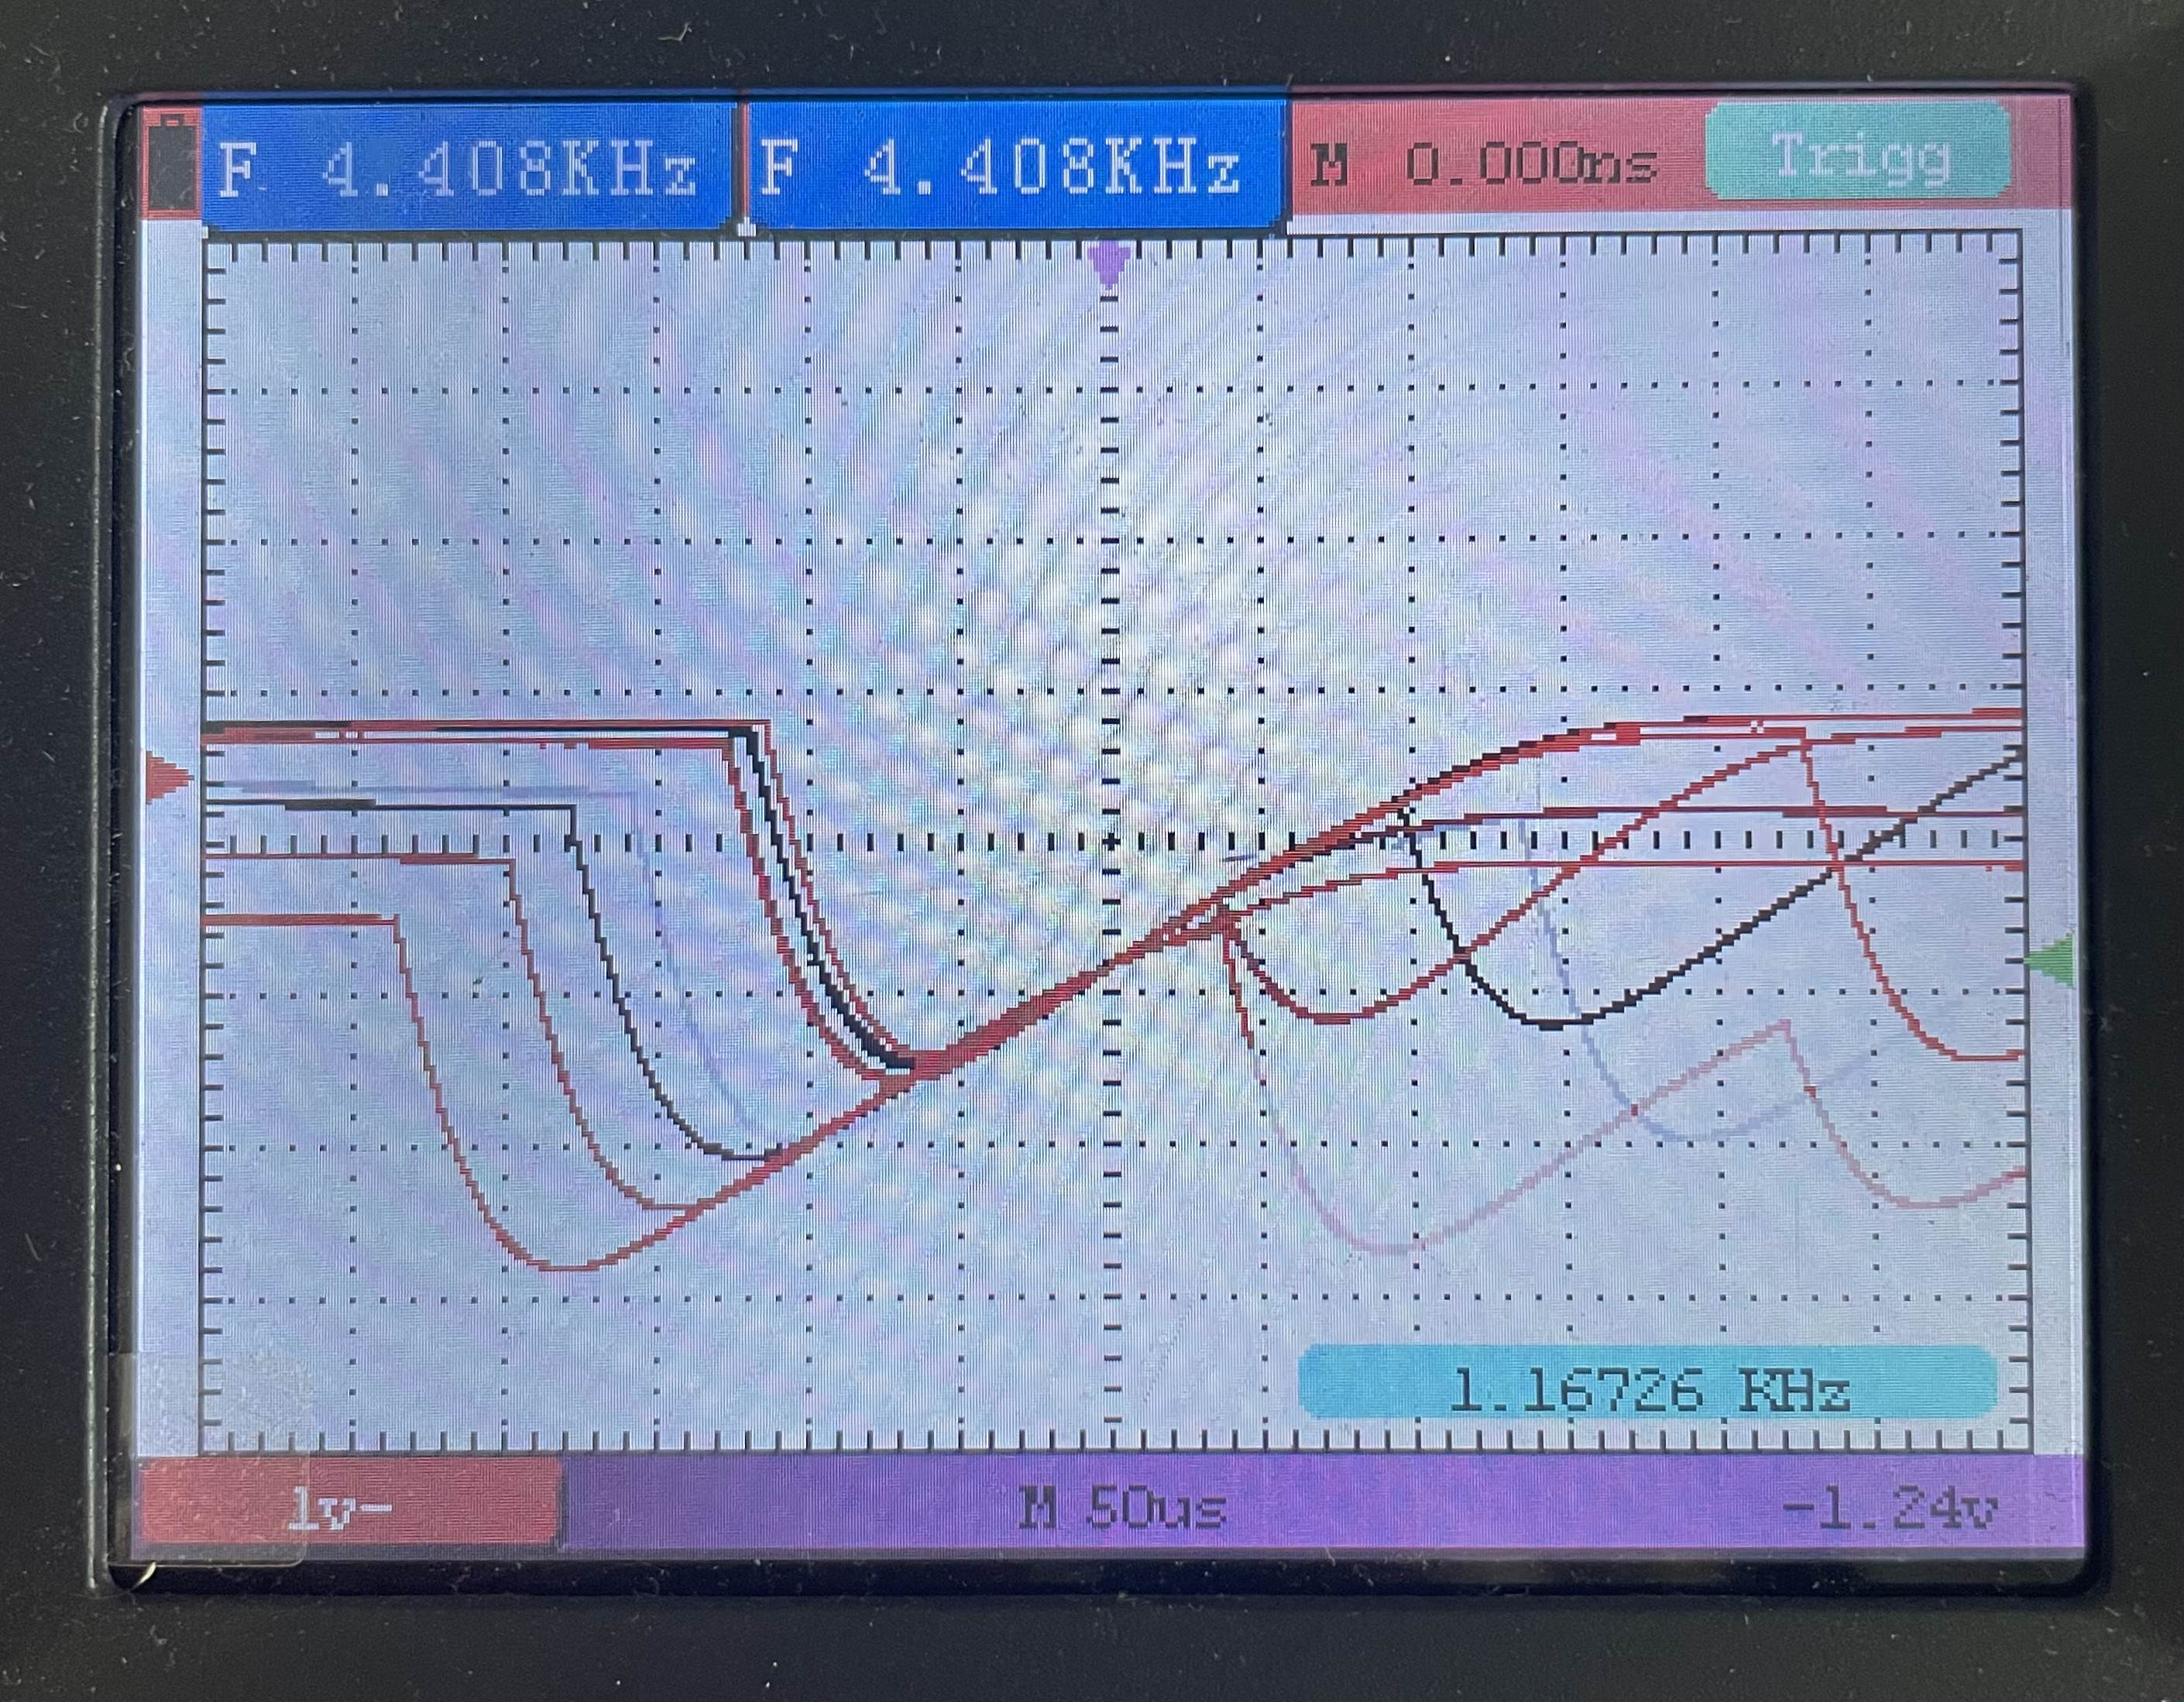
\includegraphics[width=0.6\textwidth]{content/Bilder/Totzeit.jpg}
  \caption{Totzeit und Erholungszeit am Oszilloskop.}
  \label{fig:Totzeit_Oszilloskop}
\end{figure}
Die Messdaten zur Bestimmung der Totzeit mit der zwei-Quellen-Methode sind in der Tabelle \ref{tab:Totzeit} aufgeführt. 
Daraus wird mit der Gleichung (\ref{eqn:}) die Totzeit 
$\tau _{\text{2-Quellen}} = 207,013\, \unit{\micro\second}$
berechnet.
\begin{table}[H]
  \centering
  \caption{Messdaten zur Bestimmung der Totzeit mithilfe der zwei-Quellen-Methode bei einer Messzeit von $120\,\unit{\second}$.}
  \label{tab:Totzeit}
  \begin{tblr}{colspec={c c c}}
      \toprule
      Quelle & $N\,[\unit{(120\,\second)^{-2}}]$ & $N\,[\unit{\second^{-2}}]$ \\
      \midrule
      $1$   & 193355 & 1611,292\\ 
      $2$   & 109837 & 915,308\\
      $1+2$ & 266228 & 2218,566\\
      \bottomrule
  \end{tblr}
\end{table}
Mithilfe der Totzeit und der Gleichung (\ref{eqn:}) wird die tatsächliche Zählrate 
$$N_0 = 4102,93\,\unit[per-mode=fraction]{\per\second}$$ ermittelt. Demnach ergibt sich ein Zählratenverlust von $1884,37\,\unit[per-mode=fraction]{\per\second}$.

%Siehe \autoref{fig:plot}!